\chapter{Evaluation}	
The evaluation is divided into three sections, first a section describing the web application developed, followed by one section for each framework used to develop the mobile application. In each section, the developed application, it's structure and functionality is presented, followed by the results of the code evaluation. 

\section{Web Application}
To simplify the process of making the web application compatible with web browsers as well as the mobile application, the architecture follows the Adapter pattern[INSERT REF]. The structure of the web application can be seen in figure \ref{nativewebuml}. Items within the red(blue) dotted box belong to the structure when Android SDK(PhoneGap) was used for developing the mobile application.

\begin{figure}[h!]
	\centering
    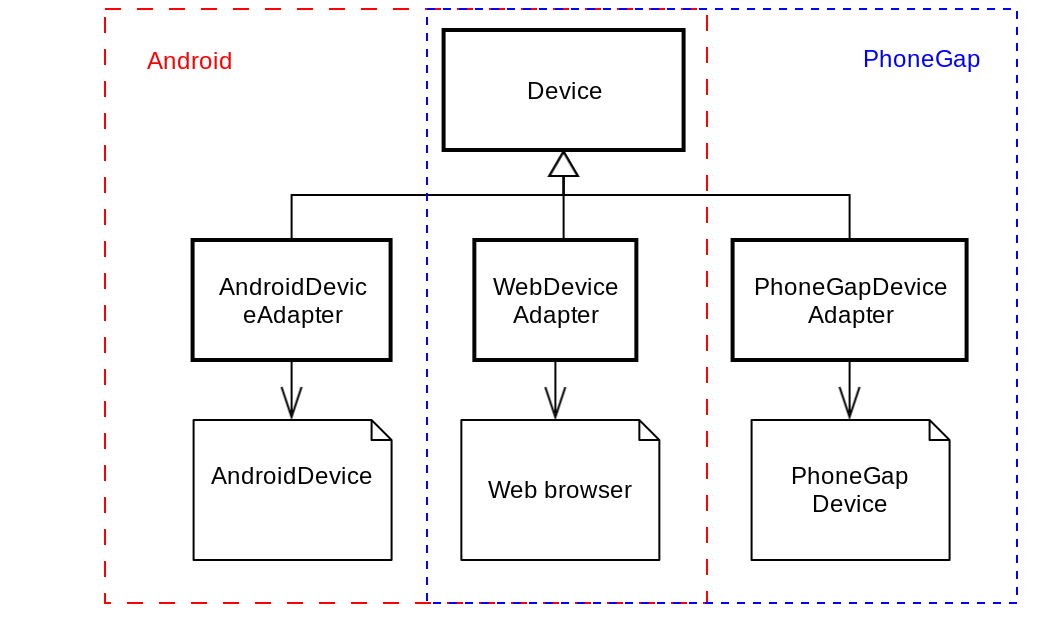
\includegraphics[width=60mm,natwidth=400,natheight=300]{./img/webuml.png}
    \caption{Structure of the web application}
	\label{fig:webuml}
\end{figure}

\section{Native android} \label{android}
The developed native application can be found on Github at [..], or in text form in the appendix. An overview of the application structure and functionality follows in section ~\ref{sec:nativestructure}. 

\subsection{Mobile Application structure} \label{sec:nativestructure}
The GUI of the Android application consist of a single WebView (used to load the web application). A UML-diagram representing the logic of the Android application can be seen in figure ~\ref{fig:nativeuml}. The contained classes are summarized below, with a short explanation followed by code examples 


\subsubsection{MainActivity} is the main Activity of the Android application. It contains logic for handling the application's Activity lifecycle, and is in charge of starting any Activities needed to provide the Web Application with data from native functions, such as the device camera. Activities are started by a call to the processIntent function. It takes an Intent and a Callback as arguments. The callback is provided a unique id, and is stored in a map. The Intent is started with the use of the startActivityForResult function provided by the Android SDK, and is assigned a request id equal to the id of the Callback. 
\\\\
	
\emph{Ex. Starting an Activity for result}
\begin{lstlisting}
// Request a unique integer to use as id
int requestCode = uniqueInteger.getUniqueInteger();

// Store the Callback in a map with the unique integer as key	
callbacks.put(requestCode, callback);
   
// Start the Activity defined in the Intent, 
// assigning the unique integer as request code
startActivityForResult(intent, requestCode);
\end{lstlisting}
	
\subsubsection{IntentFactory} provides Intents for native functions such as capturing an image or picking an image from the gallery.
	\\\\
	\emph{Ex. getting Intent from IntentFactory}
	
	\begin{lstlisting}
// In Bridge:
Intent imageIntent = IntentFactory.createCameraIntent(context);
		
// In IntentFactory:
public static Intent createCameraIntent(Context context) {
	// Create the intent for capturing an image
	Intent takePictureIntent = 
		new Intent(MediaStore.ACTION_IMAGE_CAPTURE);
	
	// Ensure that there's a camera activity to handle the intent
	if (takePictureIntent
		.resolveActivity(context.getPackageManager()) != null) {
		// Create the File where the photo should go
		File photoFile = AndroidHardware.requestImageFile();
		takePictureIntent.putExtra(MediaStore.EXTRA_OUTPUT,
		Uri.fromFile(photoFile));
	}
	return takePictureIntent;
}
\end{lstlisting}
	
\subsubsection{AndroidHardware} contains static methods, performing a single well-defined task. The code example below shows the function called to request a file for storing an image.
	\\
	\emph{Code example extracted from AndroidHardware:}
\begin{lstlisting}
public static File requestImageFile() {
 String fileName = "tempPhoto";
 File storageDir = 
   Environment.getExternalStoragePublicDirectory(
     Environment.DIRECTORY_PICTURES
     );
 File photoFile = null;
 try {
   photoFile = File.createTempFile(fileName, ".jpg", storageDir);
 } catch (IOException e) {
   e.printStackTrace();
 }
 return photoFile;
}
\end{lstlisting}
	
\subsubsection{Bridge} 
Bridge serves as a bridge between the native application and web. When the web application requests data from a native function, Bridge receives the request from JsInterface, creates the corresponding Intent and Callback, and forwards them to MainActivity, see Ex. 1 below. Bridge also receives the result from the native function call, which it forwards to WebViewDataSender, see Ex. 2 below.
\\\\
\emph{Ex. 1 Processing a request for an image from the gallery}
\begin{lstlisting}
// Create a new intent
Intent imageIntent = IntentFactory.createImageIntent(context);

// Create callback for the intent
Callback imagePickCallback = new ImagePickCallback(this, context, callback);

// Send intent to mainActivity for processing
mActivity.processIntent(imageIntent, imagePickCallback);
\end{lstlisting}

\emph{Ex. 2 Forwarding data returned from native function}
\begin{lstlisting}
public void processCallback(String callback, String argument) {
        webViewDataSender.sendData(callback, argument);
}
\end{lstlisting}
	
\subsubsection{WebViewDataSender}
WebViewDataSender is in charge of all communication with the WebView and it's encapsulated web application. Upon application start, it loads the web application and injects the JavaScriptInterface. The class also contains logic for executing JavaScript functions in the web application, used to return results from native function calls.
\emph{Ex. sendData - used by bridge to send back results to the web application}
\begin{lstlisting}
public void sendData(final String javascriptFunction, final String arg) {
        Log.d(TAG, "sendData");
        webView.post(new Runnable() {
            	@Override
            	public void run() {
        		webView.loadUrl("javascript:" + javascriptFunction + "('" + arg + "')");
    		}
	});
}
\end{lstlisting}
	
\subsubsection{JsInterface}
JsInterface is exposed to the web application as a JavaScriptInterface and acts as a receiver for function calls from the web application. If the web application requires data from a native function, the JavaScript in the web application can call upon the proper method in JsInterface, which in turn forwards the requests to Bridge.
\emph{Ex. Two java functions exposed to the web application by JsInterface}
\begin{lstlisting}
    //Request an image from the device camera
    @JavascriptInterface
    public void requestCamera(String callback) {
        Log.d(TAG, "requestImage");
        bridge.requestCamera(callback);
    }

    // Request an image from the device storage
    @JavascriptInterface
    public void requestImage(String callback) {
        Log.d(TAG, "requestImage");
        bridge.requestImage(callback);
    }
\end{lstlisting}

	
\subsubsection{Callback} 
Callback is an interface, specifying a single public method (done). Classes implementing callback contain code specifying how to send results from a requested native function call back to the web application. More specifically, the code defines which javascript function to return the data to, and how the data is to be returned. In our solution, there are two classes implementing Callback:
	\begin{description}
		\item[ImageCallback] is used when the web application requests an image from the camera
		
		\item[ImagePickCallback] is used when the web application requests an image from the gallery
	\end{description}
	
\subsubsection{UniqueInteger} 
UniqueInteger contains a single public (synchronized) function getUniqueInteger, which is guaranteed to return a unique integer on each call. This is used by MainActivity when assigning requestIds to Intents and storing their corresponding Callbacks.

\begin{figure}[h!]
	\centering
    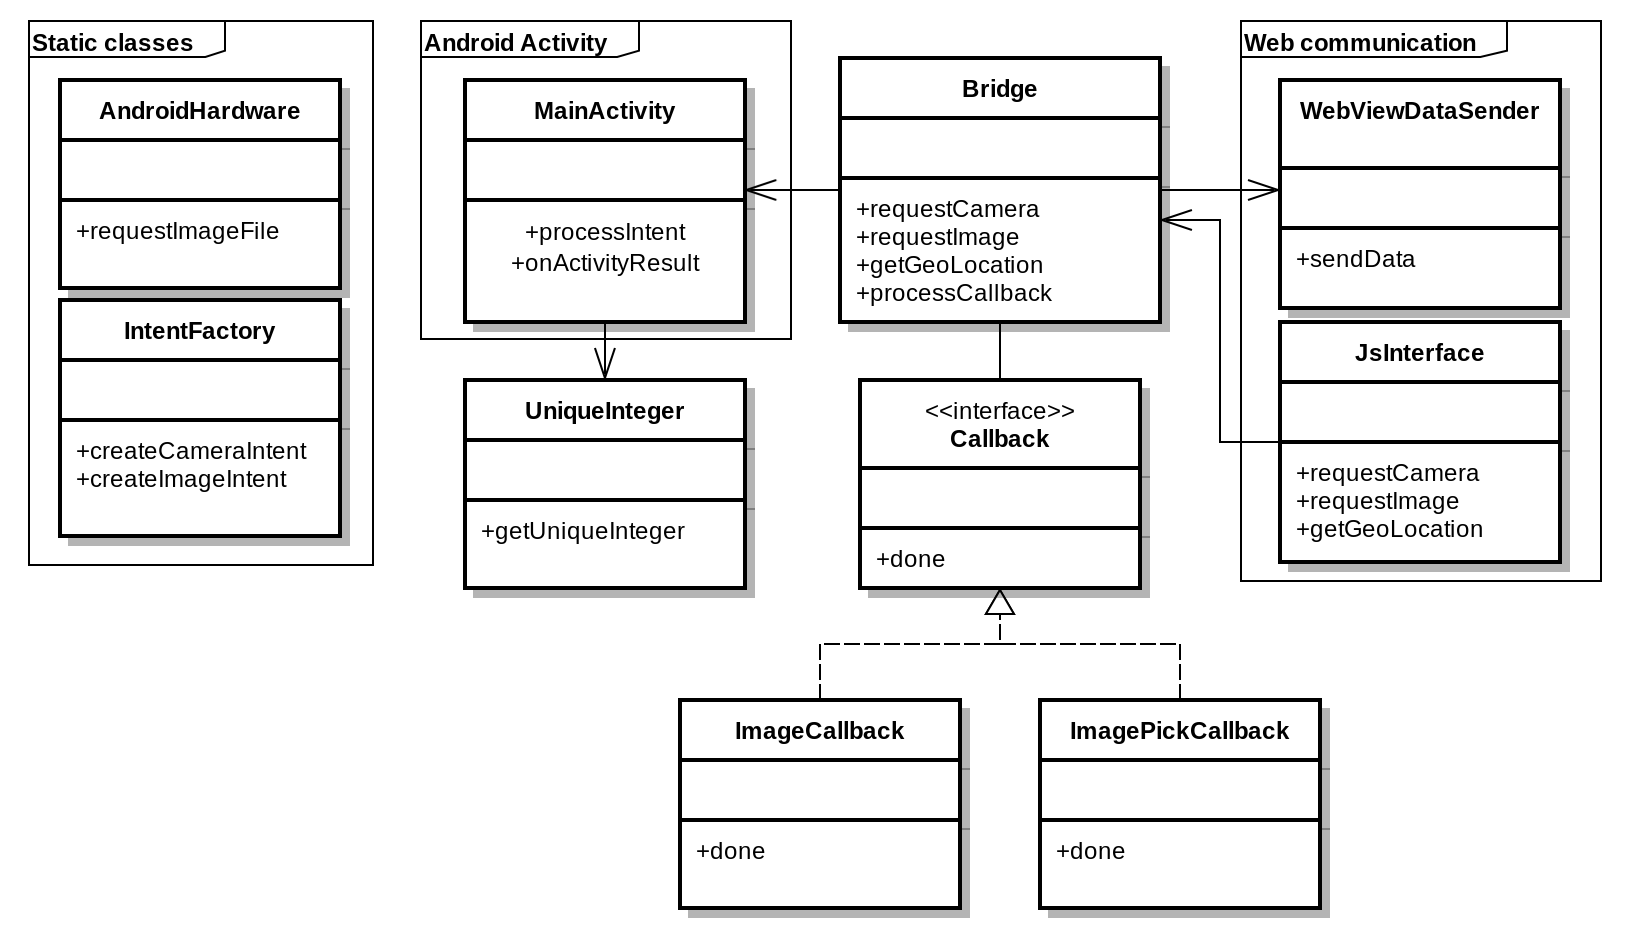
\includegraphics[width=120mm,natwidth=800,natheight=600]{./img/polluxuml.png}
    \caption{Structure of the android application}
    \label{fig:nativeuml}
\end{figure}

\subsection{Function flow} \label{sec:nativeflow}
A more detailed view of the program flow when the web application requests an image can be seen in figure ~\ref{fig:nativeflow}, further explained below.
\begin{figure}[h!]
	\centering
    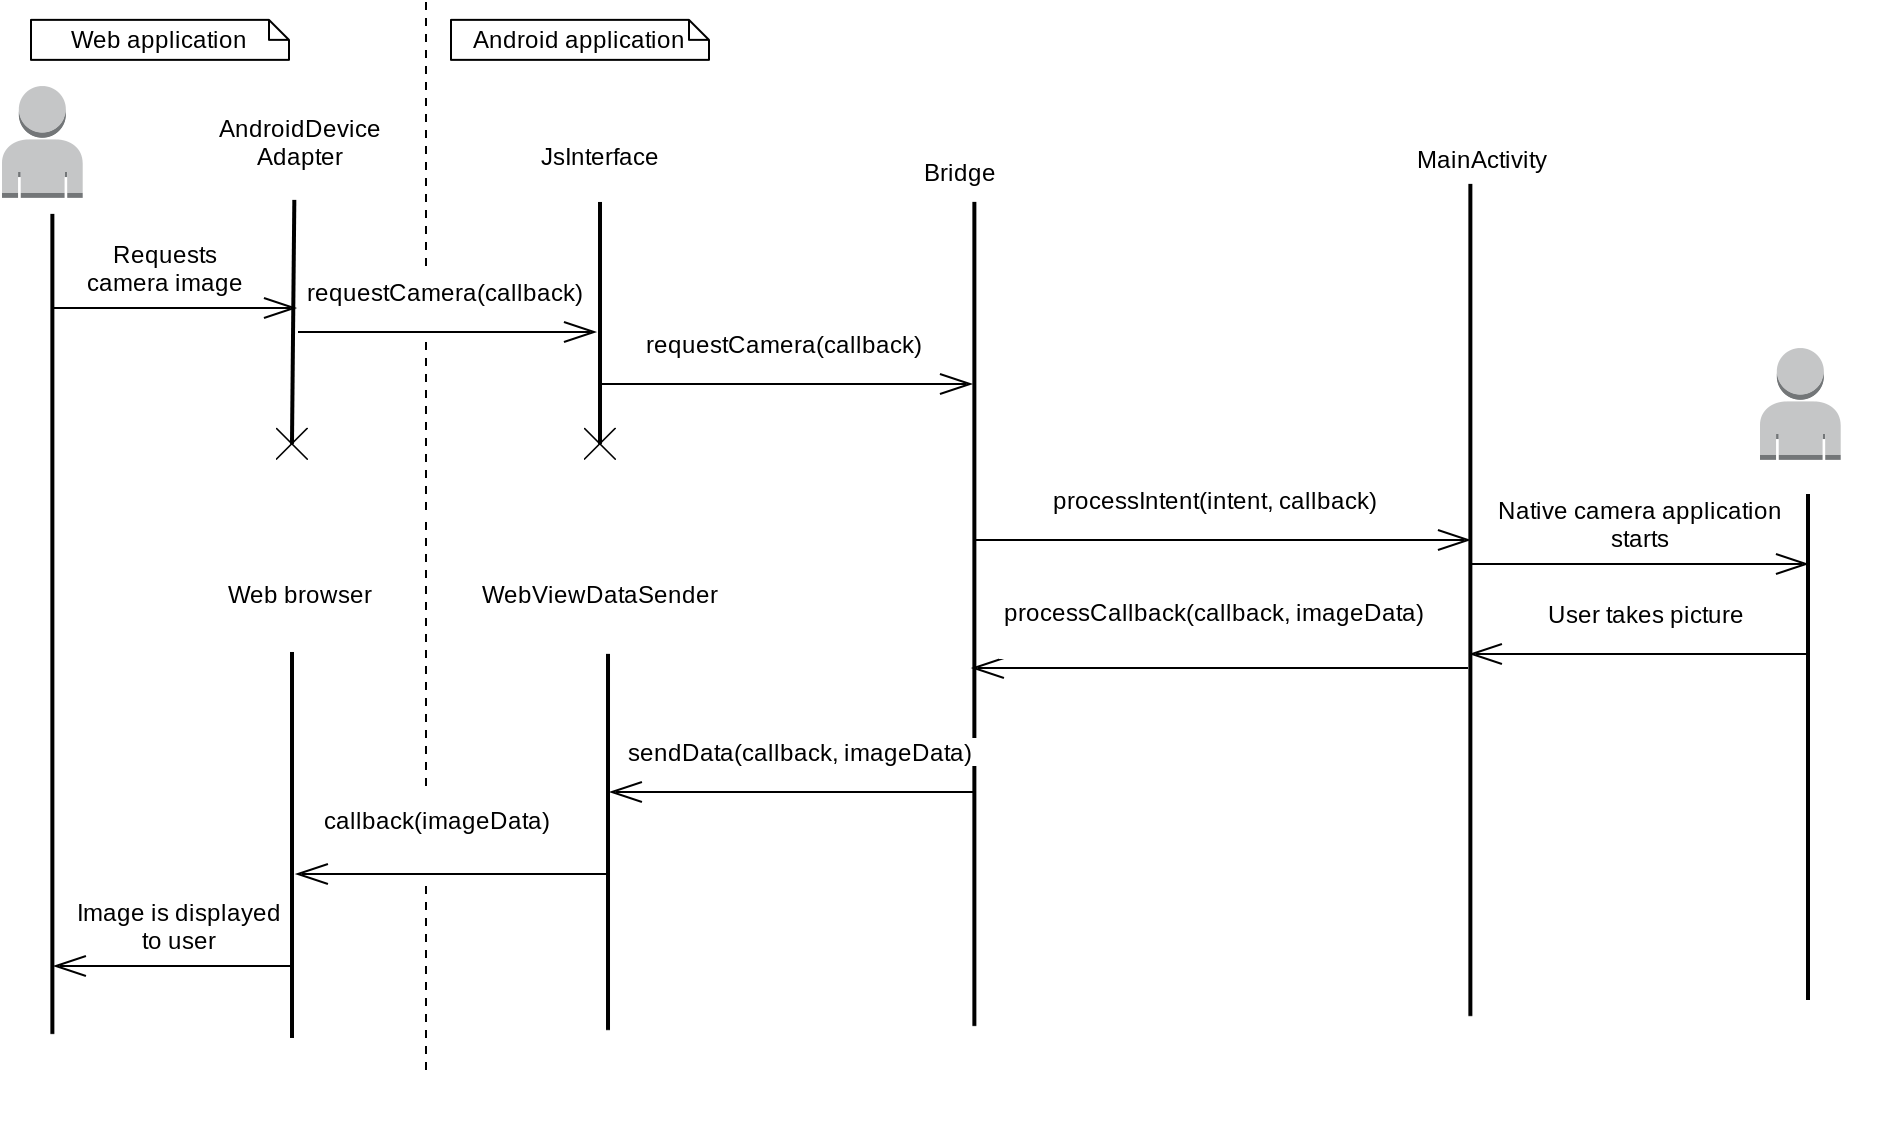
\includegraphics[width=120mm,natwidth=800,natheight=600]{./img/androidfunctionflow.png}
    \caption{Function flowchart, single call from web application}
    \label{fig:nativeflow}
\end{figure}
\begin{enumerate}
	\item User action invokes a request for an image from the mobile camera
	\item Current device adapter (AndroidDeviceAdapter) calls requestCamera on JsInterface, with the function name of the preferred callback function as argument
	\item JsInterface forwards the function call to Bridge
	\item Bridge creates the corresponding Intent and Callback, and calls processIntent on MainActivity with Intent and Callback as arguments
	\item MainActivity gets a unique id from UniqueInteger, stores the callback in a hashmap with the id as key, and starts the intent with the id as requestcode.
	\item Camera application starts
	\item When user takes a picture, MainActivity gets notified by the Android system, pulls the Callback with the same id as the processed Intent, and forwards the callback and resulting image data to Bridge through processCallback
	\item Bridge executes the callback which in turn calls sendData on WebViewDataSender, with the image data and callback name as arguments
	\item WebViewDataSender executes the JavaScript callback function in the browser window
	\item The captured image is displayed to the user in the browser
\end{enumerate}

\subsection{Code evaluation} \label{sec:nativeeval}
Evaluation of the developed application was performed as described in \ref{section-measuring-lines-of-code}, and a summary of the results  can be seen in the table below.

\begin{tabular}{ | l | c | r | }
    \hline
    \multicolumn{3}{|c|}{Quantitative metrics} \\
    \hline
	Metric & Android application &  Web application \\
	\hline
	Files & 10 & 2\\
	LLoC & 200 & 173\\	
	\hline
	\multicolumn{3}{c}{\emph{Result of code evaluation using ProjectCodeMeter}}
\end{tabular}

\section{PhoneGap}
The developed native application can be found on Github at [..], or in text form in the appendix. An overview of the application structure and functionality follows in section ~\ref{sec:phonegapstructure}, after which, the results of the code evaluation are stated in section \ref{sec:phonegapeval}

\subsection{Application structure} \label{sec:phonegapstructure}
The Android application developed using PhoneGap is a hybrid application, and is thus run within a WebView. The user interface of the developed application is a minimal HTML document containing a single inline frame, which is used to load the web application. The logic developed for the Android application is written in JavaScript, which is loaded in the WebView. A UML-diagram representing the logic of the Android application can be seen in figure ~\ref{fig:phonegapuml},  with the classes summarized below.
\begin{figure}[h!]
	\centering
    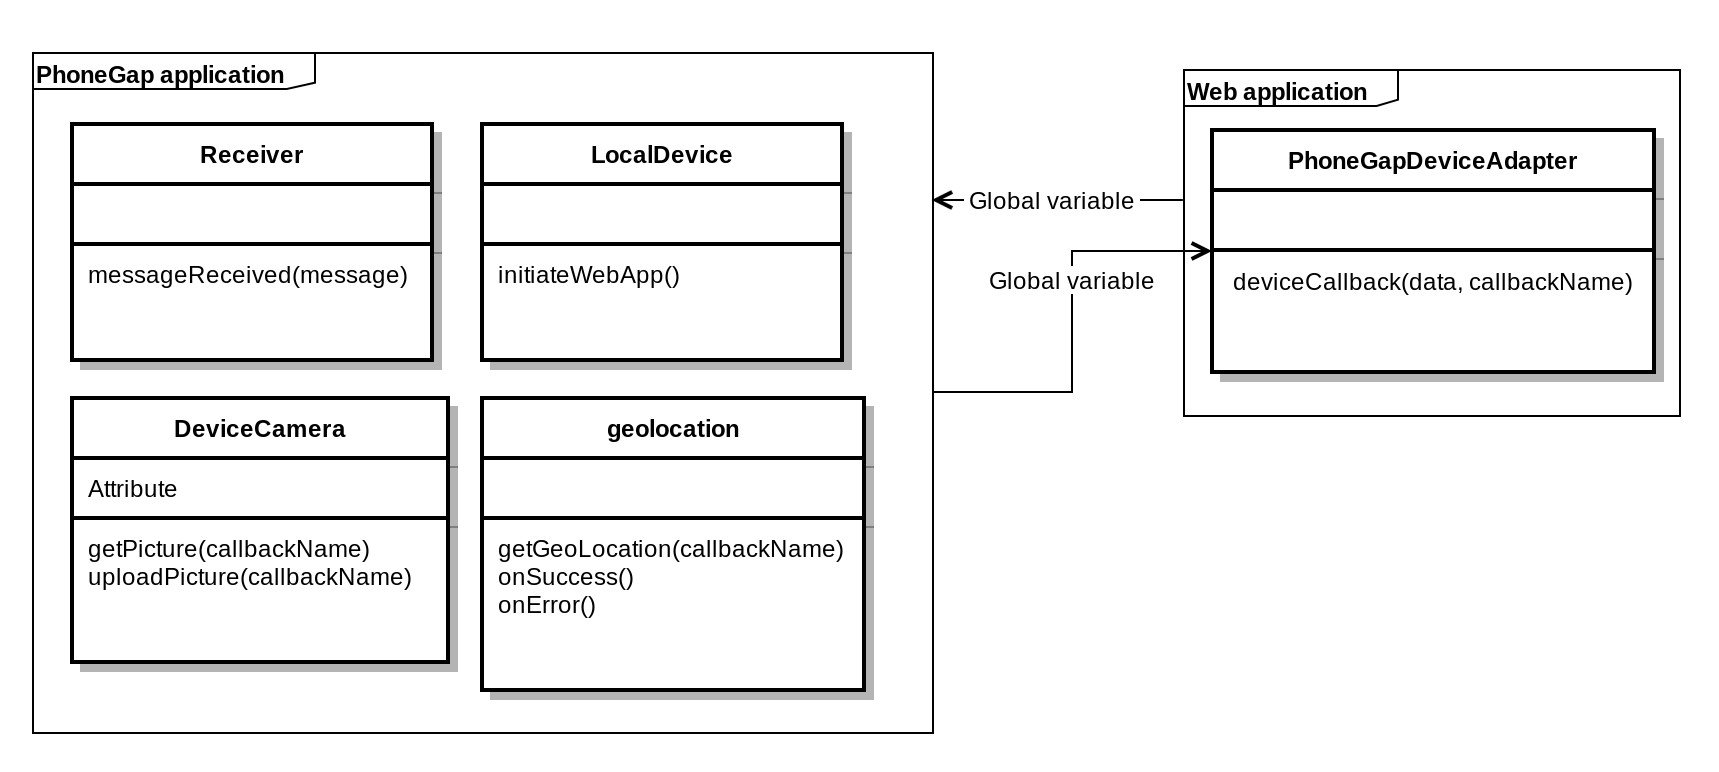
\includegraphics[width=120mm,natwidth=800,natheight=600]{./img/phonegapuml.png}
    \caption{Structure of the phonegap application}
    \label{fig:phonegapuml}
\end{figure}

\subsubsection{Receiver}
The Receiver listens to messages posted to the (HTML) window loaded in the WebView. It is used to receive messages from web application and calls the requested methods in the Android application.
\subsubsection{LocalDevice}
LocalDevice contains a single method initiateWebApp, which is used to load the web application in an inline frame and initialize device in the web application to the correct adapter.
\subsubsection{DeviceCamera}
DeviceCamera contains logic for invoking and receiving results from the device camera. It's functions are called by Reciver upon requests from the web application.
\subsubsection{geolocation}
Geolocation contains logic for accessing the mobiles geo location (GPS-position). It's functions are called by Receiver upon requests from the web application.

\subsection{Function flow}\label{sec:phonegapflow}
A more detailed view of the program flow when the web application requests an image can be seen in figure ~\ref{fig:phonegapflow}, further explained below.
\begin{figure}[h!]
	\centering
    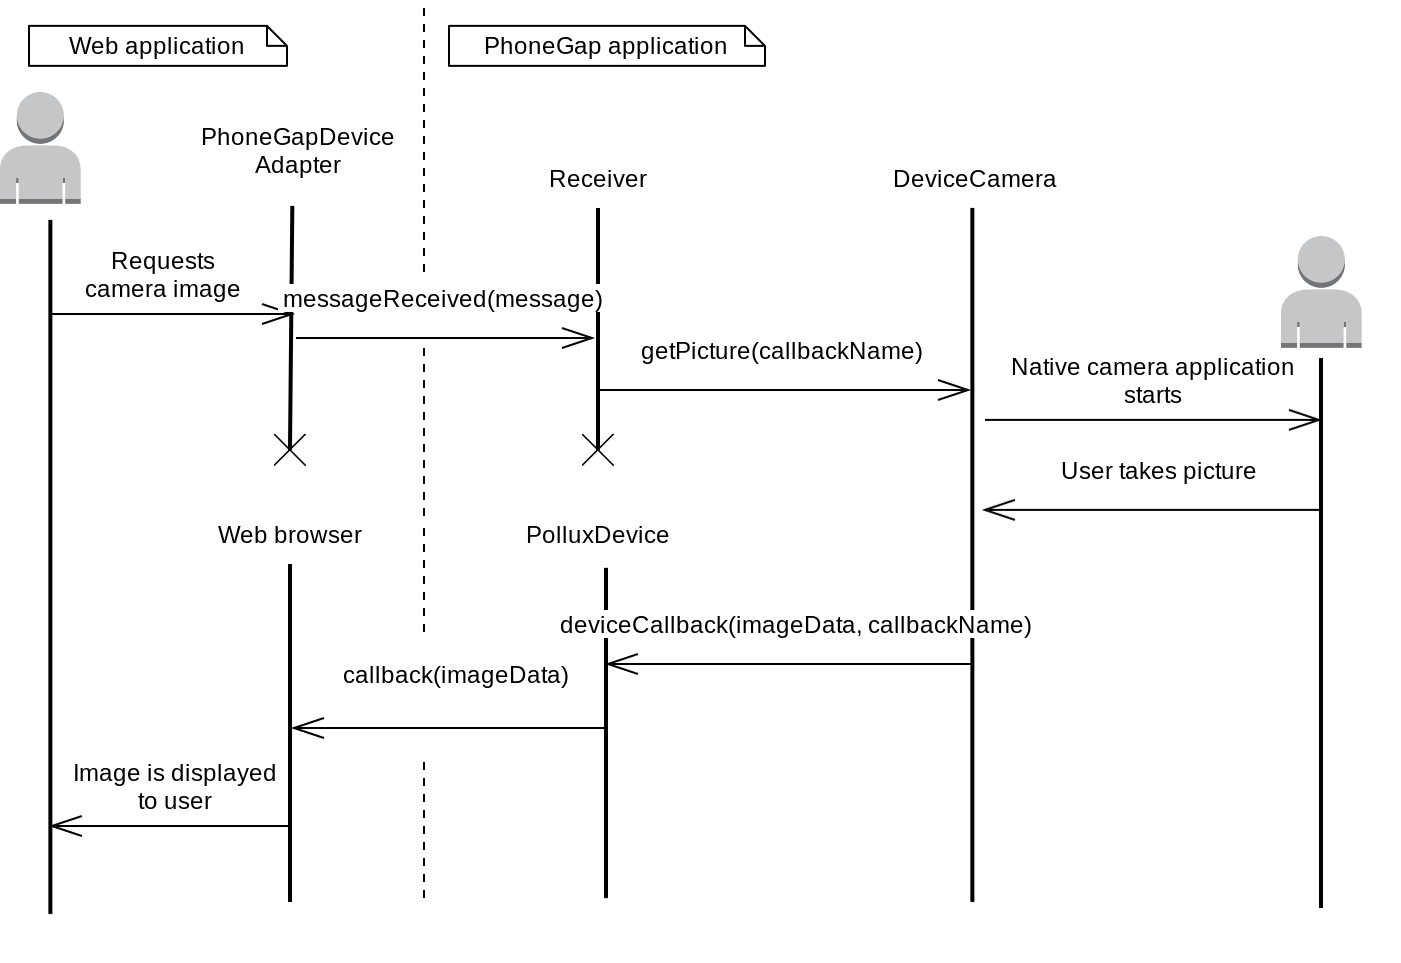
\includegraphics[width=120mm,natwidth=800,natheight=600]{./img/phonegapfunctionflow.png}
    \caption{Function flowchart, single call in web application} \label{fig:phonegapflow}
\end{figure}
\begin{enumerate}
	\item User action invokes a request for an image from the mobile camera 
	\item Current device adapter (PhoneGapDeviceAdapter) forwards the request to the PhoneGap application using postMessage
	\item The message gets processed by the PhoneGap receiver which forwards the call to DeviceCamera via the getPicture function
	\item DeviceCamera uses PhoneGap library code to start the camera application
	\item User takes picture, and the result is received by DeviceCamera
	\item DeviceCamera returns the result to the browser by invoking DeviceCallback on the exposed javascript object, in PhoneGap known as PolluxDevice
	\item DeviceCallback calls the javascript callback function specified in its argument
	\item The captured image is displayed to the user in the browser	
\end{enumerate}

\subsection{Code evaluation}\label{sec:phonegapeval}
Evaluation of the developed application was performed as described in section \ref{section-measuring-lines-of-code}, and a summary of the results  can be seen in the table below.

\begin{tabular}{ | l | c | r | }
    \hline
    \multicolumn{3}{|c|}{Quantitative metrics} \\
    \hline
	Metric & PhoneGap application &  Web application \\
	\hline
	Files & 3 & 2\\
	LLoC & 86 & 175\\	
	\hline
	\multicolumn{3}{c}{\emph{Result of code evaluation using ProjectCodeMeter}}
\end{tabular}